\documentclass[border=12pt]{standalone}
\usepackage{amssymb}
\usepackage{amsmath}
\usepackage{tikz}
\usetikzlibrary{arrows.meta, decorations.pathreplacing, calc, positioning, shapes.geometric}

% Project palette (matches covering_diagram_why_curve.tex)
\definecolor{cnavy}{HTML}{0E2747}
\definecolor{corange}{HTML}{E8573F}
\definecolor{cgreen}{HTML}{3B9B6D}
\definecolor{cslate}{HTML}{5B6680}
\definecolor{cmuted}{HTML}{9B9484}
\definecolor{ccream}{HTML}{FAFAF6}

\begin{document}
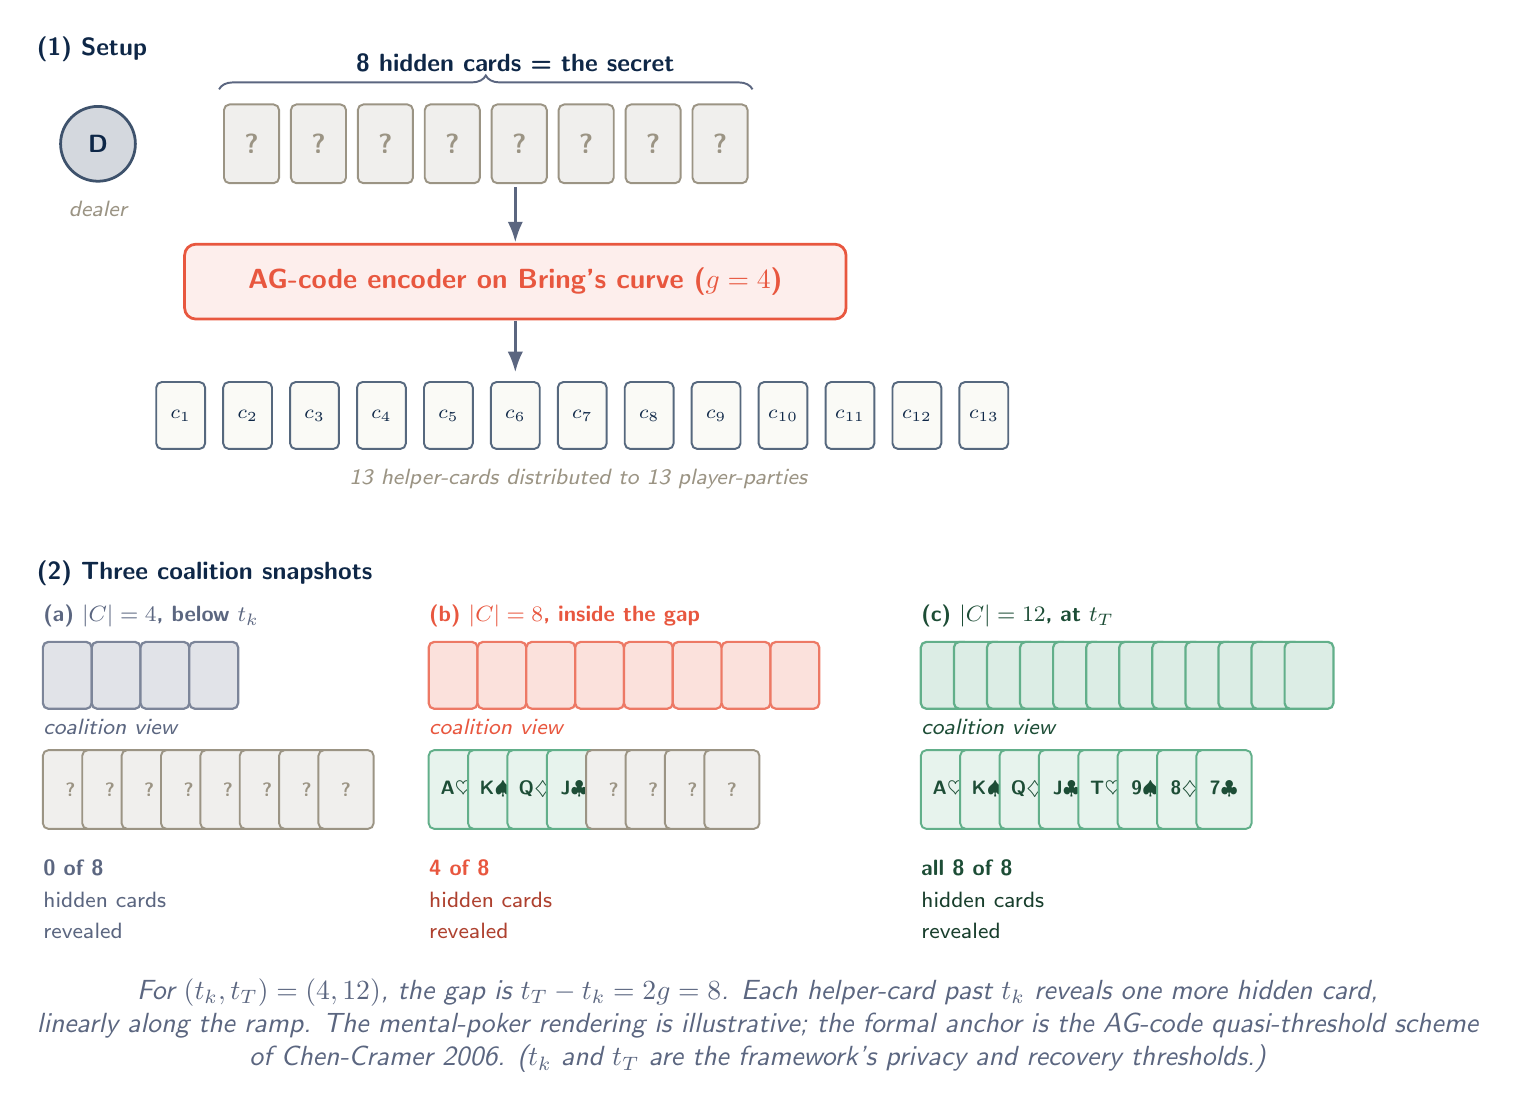
\begin{tikzpicture}[
  % Hidden card (face-down, the dealer's secret)
  hcard/.style={
    rectangle, rounded corners=2pt, draw=cmuted, fill=cmuted!15,
    line width=0.7pt, minimum width=0.70cm, minimum height=1.0cm,
    inner sep=0pt
  },
  % Hidden card after reveal (face-up)
  rcard/.style={
    rectangle, rounded corners=2pt, draw=cgreen!80, fill=cgreen!12,
    line width=0.7pt, minimum width=0.70cm, minimum height=1.0cm,
    inner sep=0pt
  },
  % Helper card (face-up, the share)
  helpercard/.style={
    rectangle, rounded corners=2pt, draw=cnavy!70, fill=ccream,
    line width=0.7pt, minimum width=0.62cm, minimum height=0.85cm,
    inner sep=0pt
  },
  helpercard-priv/.style={
    rectangle, rounded corners=2pt, draw=cslate!80, fill=cslate!18,
    line width=0.8pt, minimum width=0.62cm, minimum height=0.85cm,
    inner sep=0pt
  },
  helpercard-gap/.style={
    rectangle, rounded corners=2pt, draw=corange!80, fill=corange!18,
    line width=0.8pt, minimum width=0.62cm, minimum height=0.85cm,
    inner sep=0pt
  },
  helpercard-rec/.style={
    rectangle, rounded corners=2pt, draw=cgreen!80, fill=cgreen!18,
    line width=0.8pt, minimum width=0.62cm, minimum height=0.85cm,
    inner sep=0pt
  },
  encoder/.style={
    rectangle, rounded corners=4pt, draw=corange, fill=corange!10,
    line width=1.0pt, minimum width=8.4cm, minimum height=0.95cm,
    inner sep=6pt
  },
  dealer/.style={
    circle, draw=cnavy!80, fill=cnavy!18, line width=1.0pt,
    minimum size=0.95cm, inner sep=0pt
  },
  font=\sffamily
]

% ============================================================
% Panel 1 (top): "Setup"
% ============================================================
\node[cnavy, font=\sffamily\bfseries\small, anchor=west] at (-0.6, 12.5)
  {(1) Setup};

% Dealer on the left
\node[dealer] (D) at (0.3, 11.3) {};
\node[cnavy, font=\sffamily\bfseries\small] at (0.3, 11.3) {D};
\node[cmuted, font=\sffamily\itshape\footnotesize, anchor=north] at (0.3, 10.7)
  {dealer};

% 8 hidden cards (the secret), to the right of the dealer
\foreach \i in {1,...,8} {
  \node[hcard] (h\i) at (1.4 + 0.85*\i, 11.3) {};
  \node[cmuted, font=\sffamily\bfseries] at (1.4 + 0.85*\i, 11.3) {?};
}

% Brace + label above the 8 hidden cards
\draw[decorate, decoration={brace, amplitude=5pt}, line width=0.7pt, draw=cslate]
  ($(h1.north west)+(-0.05,0.18)$) -- ($(h8.north east)+(0.05,0.18)$);
\node[cnavy, font=\sffamily\bfseries\small, anchor=south] at (5.6, 12.10)
  {8 hidden cards = the secret};

% Arrow down to encoder
\draw[-{Latex[length=2.6mm]}, draw=cslate, line width=0.9pt]
  (5.6, 10.75) -- (5.6, 10.05);

% Encoder block
\node[encoder] (E) at (5.6, 9.55) {};
\node[corange, font=\sffamily\bfseries] at (5.6, 9.55)
  {AG-code encoder on Bring's curve ($g=4$)};

% Arrow down to helper-cards
\draw[-{Latex[length=2.6mm]}, draw=cslate, line width=0.9pt]
  (5.6, 9.05) -- (5.6, 8.40);

% 13 helper-cards (the shares)
\foreach \i in {1,...,13} {
  \node[helpercard] (s\i) at (0.5 + 0.85*\i, 7.85) {};
  \node[cnavy, font=\sffamily\bfseries\scriptsize] at (0.5 + 0.85*\i, 7.85) {$c_{\i}$};
}

% Caption under helper-cards
\node[cmuted, font=\sffamily\itshape\footnotesize] at (6.4, 7.05)
  {13 helper-cards distributed to 13 player-parties};

% ============================================================
% Panel 2 (middle): "Three coalition snapshots"
% ============================================================
\node[cnavy, font=\sffamily\bfseries\small, anchor=west] at (-0.6, 5.85)
  {(2) Three coalition snapshots};

% Common Y baseline for the helper-card subset:  y = 4.55
% Below it: 8 hidden cards in their state, baseline  y = 3.10
% Captions  y = 2.10

% --------------------------------------
% (a) Privacy zone: |C| = 4, below ts_k
% Block-left X = -0.4; first card LEFT edges aligned to that X.
% --------------------------------------
\node[cslate, font=\sffamily\bfseries\footnotesize, anchor=west, inner xsep=0pt] at (-0.4, 5.30)
  {(a) $|C|=4$, below $t_k$};

% 4 helper-cards in privacy style: first center at -0.4 + 0.31 = -0.09
\foreach \i in {1,...,4} {
  \node[helpercard-priv] at (-0.71 + 0.62*\i, 4.55) {};
}
\node[cslate, font=\sffamily\itshape\footnotesize, anchor=west, inner xsep=0pt] at (-0.4, 3.90)
  {coalition view};
% 8 hidden cards (still face-down): first center at -0.4 + 0.35 = -0.05
\foreach \i in {1,...,8} {
  \node[hcard] at (-0.55 + 0.50*\i, 3.10) {};
  \node[cmuted, font=\sffamily\bfseries\scriptsize] at (-0.55 + 0.50*\i, 3.10) {?};
}
% Caption
\node[cslate, font=\sffamily\bfseries\footnotesize, align=left, anchor=west, inner xsep=0pt]
  at (-0.4, 2.10) {\textbf{0 of 8}};
\node[cslate, font=\sffamily\footnotesize, align=left, anchor=west, inner xsep=0pt]
  at (-0.4, 1.70) {hidden cards};
\node[cslate, font=\sffamily\footnotesize, align=left, anchor=west, inner xsep=0pt]
  at (-0.4, 1.30) {revealed};

% --------------------------------------
% (b) Gap zone: |C| = 8, between
% Block-left X = 4.5; first card LEFT edges aligned to that X.
% helper-card width 0.62, so first center = 4.5 + 0.31 = 4.81 => +0.62*i with offset 4.19
% hidden card width 0.70, so first center = 4.5 + 0.35 = 4.85 => +0.50*i with offset 4.35
% --------------------------------------
\node[corange, font=\sffamily\bfseries\footnotesize, anchor=west, inner xsep=0pt] at (4.5, 5.30)
  {(b) $|C|=8$, inside the gap};

% 8 helper-cards in gap style
\foreach \i in {1,...,8} {
  \node[helpercard-gap] at (4.19 + 0.62*\i, 4.55) {};
}
\node[corange, font=\sffamily\itshape\footnotesize, anchor=west, inner xsep=0pt] at (4.5, 3.90)
  {coalition view};
% 8 hidden cards: 4 revealed (face-up with rank labels), 4 still face-down
\node[rcard] at (4.35 + 0.50*1, 3.10) {};
  \node[cgreen!50!black, font=\sffamily\bfseries\scriptsize] at (4.35 + 0.50*1, 3.10) {A$\heartsuit$};
\node[rcard] at (4.35 + 0.50*2, 3.10) {};
  \node[cgreen!50!black, font=\sffamily\bfseries\scriptsize] at (4.35 + 0.50*2, 3.10) {K$\spadesuit$};
\node[rcard] at (4.35 + 0.50*3, 3.10) {};
  \node[cgreen!50!black, font=\sffamily\bfseries\scriptsize] at (4.35 + 0.50*3, 3.10) {Q$\diamondsuit$};
\node[rcard] at (4.35 + 0.50*4, 3.10) {};
  \node[cgreen!50!black, font=\sffamily\bfseries\scriptsize] at (4.35 + 0.50*4, 3.10) {J$\clubsuit$};
\foreach \i in {5,...,8} {
  \node[hcard] at (4.35 + 0.50*\i, 3.10) {};
  \node[cmuted, font=\sffamily\bfseries\scriptsize] at (4.35 + 0.50*\i, 3.10) {?};
}
% Caption
\node[corange, font=\sffamily\bfseries\footnotesize, align=left, anchor=west, inner xsep=0pt]
  at (4.5, 2.10) {\textbf{4 of 8}};
\node[corange!75!black, font=\sffamily\footnotesize, align=left, anchor=west, inner xsep=0pt]
  at (4.5, 1.70) {hidden cards};
\node[corange!75!black, font=\sffamily\footnotesize, align=left, anchor=west, inner xsep=0pt]
  at (4.5, 1.30) {revealed};

% --------------------------------------
% (c) Recovery zone: |C| = 12, at ts_T
% Block-left X = 10.75; first card LEFT edges aligned to that X.
% helper-card width 0.62, so first center = 10.75 + 0.31 = 11.06 => +0.42*i with offset 10.64
% hidden card width 0.70, so first center = 10.75 + 0.35 = 11.10 => +0.50*i with offset 10.60
% --------------------------------------
\node[cgreen!50!black, font=\sffamily\bfseries\footnotesize, anchor=west, inner xsep=0pt] at (10.75, 5.30)
  {(c) $|C|=12$, at $t_T$};

% 12 helper-cards in recovery style
\foreach \i in {1,...,12} {
  \node[helpercard-rec] at (10.64 + 0.42*\i, 4.55) {};
}
\node[cgreen!50!black, font=\sffamily\itshape\footnotesize, anchor=west, inner xsep=0pt] at (10.75, 3.90)
  {coalition view};
% All 8 hidden cards revealed (face-up)
\node[rcard] at (10.60 + 0.50*1, 3.10) {};
  \node[cgreen!50!black, font=\sffamily\bfseries\scriptsize] at (10.60 + 0.50*1, 3.10) {A$\heartsuit$};
\node[rcard] at (10.60 + 0.50*2, 3.10) {};
  \node[cgreen!50!black, font=\sffamily\bfseries\scriptsize] at (10.60 + 0.50*2, 3.10) {K$\spadesuit$};
\node[rcard] at (10.60 + 0.50*3, 3.10) {};
  \node[cgreen!50!black, font=\sffamily\bfseries\scriptsize] at (10.60 + 0.50*3, 3.10) {Q$\diamondsuit$};
\node[rcard] at (10.60 + 0.50*4, 3.10) {};
  \node[cgreen!50!black, font=\sffamily\bfseries\scriptsize] at (10.60 + 0.50*4, 3.10) {J$\clubsuit$};
\node[rcard] at (10.60 + 0.50*5, 3.10) {};
  \node[cgreen!50!black, font=\sffamily\bfseries\scriptsize] at (10.60 + 0.50*5, 3.10) {T$\heartsuit$};
\node[rcard] at (10.60 + 0.50*6, 3.10) {};
  \node[cgreen!50!black, font=\sffamily\bfseries\scriptsize] at (10.60 + 0.50*6, 3.10) {9$\spadesuit$};
\node[rcard] at (10.60 + 0.50*7, 3.10) {};
  \node[cgreen!50!black, font=\sffamily\bfseries\scriptsize] at (10.60 + 0.50*7, 3.10) {8$\diamondsuit$};
\node[rcard] at (10.60 + 0.50*8, 3.10) {};
  \node[cgreen!50!black, font=\sffamily\bfseries\scriptsize] at (10.60 + 0.50*8, 3.10) {7$\clubsuit$};
% Caption
\node[cgreen!50!black, font=\sffamily\bfseries\footnotesize, align=left, anchor=west, inner xsep=0pt]
  at (10.75, 2.10) {\textbf{all 8 of 8}};
\node[cgreen!40!black, font=\sffamily\footnotesize, align=left, anchor=west, inner xsep=0pt]
  at (10.75, 1.70) {hidden cards};
\node[cgreen!40!black, font=\sffamily\footnotesize, align=left, anchor=west, inner xsep=0pt]
  at (10.75, 1.30) {revealed};

% ============================================================
% Panel 3 (bottom): Caption
% ============================================================
\node[cslate, font=\sffamily\itshape, align=center, anchor=west] at (-0.6, 0.1) {
  For $(t_k, t_T)=(4,12)$, the gap is $t_T-t_k = 2g = 8$.
  Each helper-card past $t_k$ reveals one more hidden card,\\
  linearly along the ramp. The mental-poker rendering is illustrative;
  the formal anchor is the AG-code quasi-threshold scheme\\
  of Chen-Cramer 2006. ($t_k$ and $t_T$ are the framework's
  privacy and recovery thresholds.)
};

\end{tikzpicture}
\end{document}
